\documentclass[hyperref={unicode}]{beamer}
%
% Choose how your presentation looks.
%
% For more themes, color themes and font themes, see:
% http://deic.uab.es/~iblanes/beamer_gallery/index_by_theme.html
%
\mode<presentation>
{
  \usetheme{default}      % or try Darmstadt, Madrid, Warsaw, ...
  \usecolortheme{default} % or try albatross, beaver, crane, ...
  \usefonttheme{default}  % or try serif, structurebold, ...
  \setbeamertemplate{navigation symbols}{}
  \setbeamertemplate{caption}[numbered]
} 
\usepackage[czech]{babel}
\usepackage{siunitx}
\usepackage[utf8]{inputenc}

\title[prezentace]{VPython/GlowScript Trinket ve výuce fyziky}
\author{Aliaksei Kalosha}
\institute{TUL}
\date{\today}

\begin{document}
\begin{frame}
  \titlepage
\end{frame}

\begin{frame}{Seznam kapitol}
    \tableofcontents
\end{frame}

\section{Úvod}
\begin{frame}
    \frametitle{Úvod}
    ~V~současné době, se klade velký důraz na vizualizaci všech abstraktních pojmů, jak ve vzdělávání, tak~i~v běžném životě. Tento fakt je učitelům fyziky dávno znám. Proto je nekolik řešení
    \begin{itemize}
        \item Někteří učitelé svým žákům~a~studentům svoje vlastní vizualizace nabízí/vytváří.
        \item Použít vizualizační programy od specializovaných vzdělávacích firem.
    \end{itemize}
   Cílem tohoto příspěvku je představit jedno takové prostředí, ve kterém mohou jak učitelé, tak~i~žáci, zdarma~a~na různých platformách vytvářet fyzikální vizualizace.
\end{frame}

\section{Prezentace}
\subsection{Úkazka dat z fyziky}
\begin{frame}
    \frametitle{Úkazka dat z fyziky}
     \begin{figure}
        \centering
        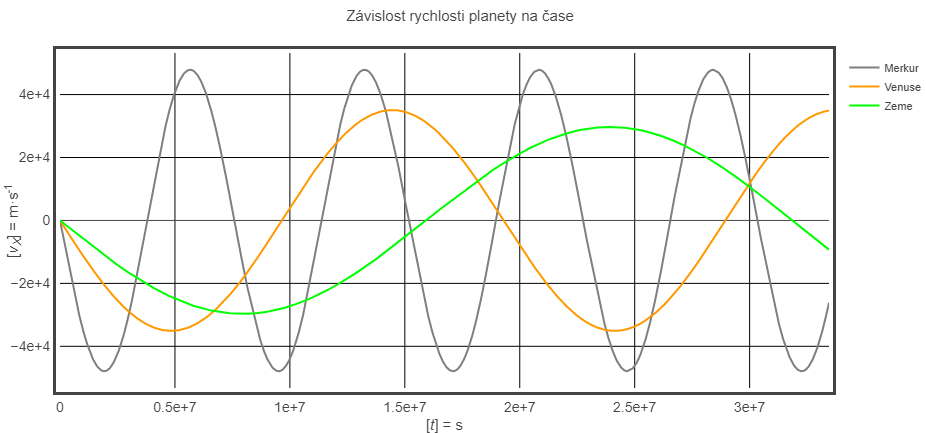
\includegraphics[width=\textwidth]{img1.png}
        %\caption{Caption}
        %\label{fig:my_label}
    \end{figure}
    Graf je težce pochopitelný~a~proto není nejlepší pro žáky.
\end{frame}
\subsection{Jak vypadá UI}
\begin{frame}
    \frametitle{Jak vypadá UI}
    \begin{figure}
        \centering
        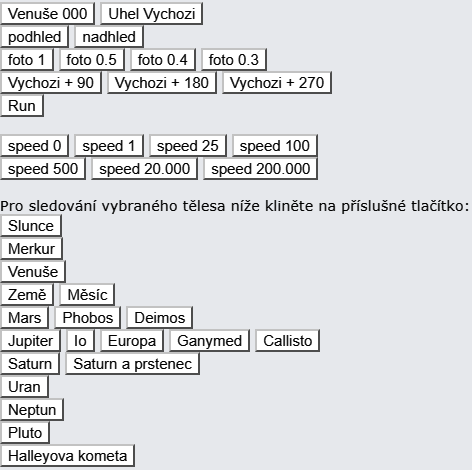
\includegraphics[width=0.5\textwidth]{img4.png}
        %\caption{Caption}
        %\label{fig:my_label}
    \end{figure}
    
    Žáci můžou samostatně vyzkoušet simulace systému~a~proto mít větší zájem~o~fyziku.
\end{frame}

\subsection{Simulace}
\begin{frame}
    \frametitle{Simulace}
    \begin{figure}
        \centering
        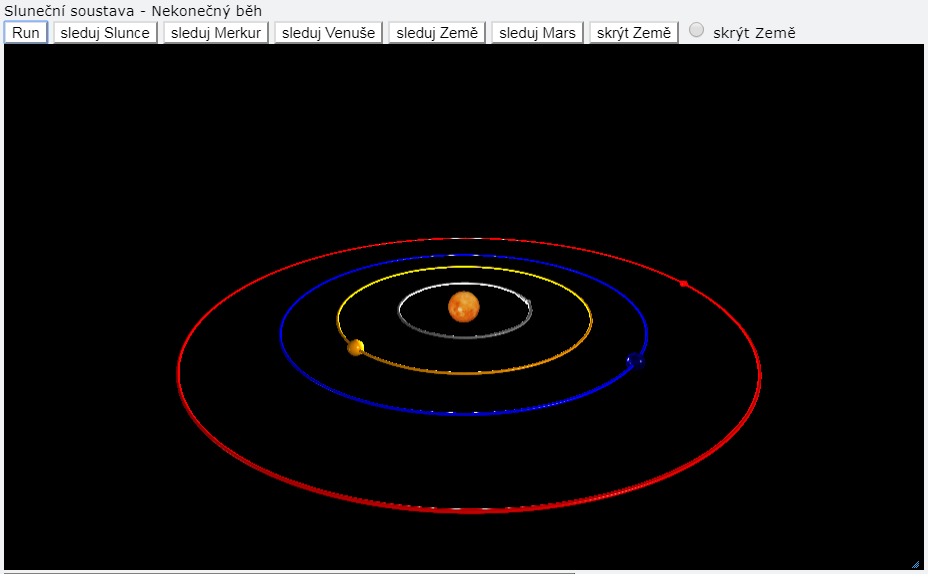
\includegraphics[width=\textwidth]{img3.png}
        %\caption{Caption}
        %\label{fig:my_label}
    \end{figure}
    Ukázka samotního programu.
\end{frame}
\section{Závěr}
\begin{frame}
\frametitle{Závěr}
~O~te aplikaci by se dalo říct : 
\begin{itemize}
    \item Tvorba modelů pro výuku fyziky~v~prostředí GlowScript Trinket není nijak náročná.
    \item ~Z~pohledu žáka je vytvořený model názorný~a~může~s~ním manipulovat tak, aby došel kompletního pochopení probíraných pojmů. 
    \item Výhodou předloženého prostředí je absolutní nezávislost na platformě~a~není potřeba instalovat žádný další software.
\end{itemize}
\end{frame}
\end{document}
